\documentclass[12pt,a4paper,oneside]{scrbook}
\usepackage[spanish]{babel}
\usepackage[utf8]{inputenc}
\usepackage[T1]{fontenc}
\usepackage{mathpazo}
\usepackage{amsmath,amsfonts,amssymb,latexsym}
\usepackage{graphicx}

\usepackage{listings}
\usepackage{xcolor}

\definecolor{miverde}{rgb}{0,0.6,0}
\definecolor{migris}{rgb}{0.5,0.5,0.5}

\lstset{
  backgroundcolor=\color{yellow!20!white},
  basicstyle=\footnotesize\ttfamily,
  breakatwhitespace=false,
  breaklines=true,
  captionpos=b,
  commentstyle=\color{miverde},
  deletekeywords={...},
  escapeinside={\%*}{*)},
  extendedchars=true,
  frame=lrtb,
  keepspaces=true,
  keywordstyle=\color{blue},
  language=Python,
  otherkeywords={*,...},
  numbers=left,
  numbersep=10pt,
  numberstyle=\small\color{migris},
  rulecolor=\color{black},
  showspaces=false,
  showstringspaces=false,
  showtabs=true,
  stepnumber=1,
  stringstyle=\color{red},
  tabsize=4,
  title=\lstname 
  }
\usepackage{tikz, pgfplots}
\pgfplotsset{width=10cm,compat=1.9}
%\usepgfplotslibrary{external}
%\tikzexternalize

% Referencias - Enlaces
%\usepackage[hyphens]{url}
\usepackage[breaklinks,bookmarks=true,colorlinks=true,linkcolor=black,
citecolor=red, urlcolor=blue]{hyperref}
\usepackage[all]{hypcap}

\usepackage{caption}
\captionsetup{font=small,format=plain,parskip=1pt,justification=centering}
\setcounter{chapter}{0}


\usepackage[total={18cm,21cm},left=2cm,top=2cm]{geometry}
\parindent=0mm
\renewcommand{\baselinestretch }{1.2}
\usepackage{icomma} 
\usepackage{fancyhdr} %activamos el paquete
\usepackage{endnotes} 
\usepackage[superscript]{cite} %las citas

\renewcommand\citeform[1]{\textcolor{blue}{#1}}  % Ponemos las citas en azul

\let\footnote=\endnote
\def\footnotetext{\endnotetext[\number\numexpr\value{endnote}+1]}
\let\footnotemark\endnotemark

\pagestyle{fancy} %seleccionamos un estilo
\lhead{Interpolación Polinómica} %texto izquierda de la cabecera
\rhead{\thepage }
\chead{Interpolación} %texto centro de la cabecera
\rfoot{Interpolación} %texto izquierda del pie
\rhead{\thepage } %número de página a la derecha
\renewcommand{\footrulewidth}{0.4pt} 
\renewcommand{\headrulewidth}{0.4pt}

\setcounter{secnumdepth}{0}
\setcounter{tocdepth}{1}

\newcounter{ns}
\addtocounter{ns}{1} 


\title{Interpolación}
\author{Cristóbal López Silla\\ Lic. En Matemáticas }
\date{Abril 2020}

\begin{document}
\maketitle
\tableofcontents
\clearpage

\section{Presentación}
Hola, e intentado hacer un compendio sobre los distintos métodos para interpolar y extrapolar funciones o valores. Esta breve recopilación va al grano, no me detengo en demostrar teoremas, propiedades, etc; mas bien las expongo. Todos los métodos vienen con su respectivo código escrito en lenguaje Python. Estos códigos los puedes cambiar a tu antojo, no hay ningún tipo de restricción de licencia. Los programas han sido creados por mi, a partir de pseudocódigos basados en libros de texto orientados a Métodos Numéricos.
\section{Introducción}
Si tenemos una función matemática no polinómica con una expresión analítica no sencilla, y con ella vamos a realizar muchos cálculos; es conveniente poder obtener una expresión analítica más sencilla, generalmente un polinomio de grado n. Para obtener el polinomio podemos aplicar métodos como los explicados aquí. Algunos métodos utilizan la información de la derivada, como los métodos spline.\\
Pero también puede ocurrir que no conozcamos la expresión analítica de la función, si no que lo que tenemos son una tabla de valores. En este caso queremos calcular un función que se aproxime lo más posible a los datos de la tabla. Se hace mediante métodos como los aquí vistos.\\
A partir de una tabla de datos, podemos querer averiguar información sobre datos que pertenecerían al interior de la tabla, en este caso lo que hacemos es \textbf{Interpolar}. Si queremos averiguar datos no pertenecientes a la tabla lo que hacemos es \textbf{Extrapolar}. La extrapolación sólo es conveniente realizarla para datos externos que estén muy cercanos a los datos extremos de la tabla. Esto es debido a que al calcular el polinomio, el susodicho polinomio aproxima muy bien a los datos que conocemos y a los muy cercanos a ellos.\\
Esta humilde guía empieza con los polinomios interpolación de Lagrange, por ser el punto de partida de los demás métodos, los cuales mejoran el tiempo computacional, la reunión de información previa, o la obtención del mejor polinomio interpolador.\\
He introducido las curvas Bézier para que tengas en perspectiva lo importantes que son en cosas como dibujo asistido en ordenador, tratamiento de imágenes, etc.

\section{Polinomios De Interpolación De Lagrange}
Consideraremos una función cualquiera $f:[a,b]\rightarrow\mathbb{R}$, dicha función cumple que $f\in\mathbf{C}^{n+1}([a,b])$.\\
Tomemos una partición de puntos distintos dos a dos, $\{ x_0,x_1,...,x_n \} \subset [a,b]$.\\
Nuestro objetivo es encontrar un polinomio de grado $\leq n$ que se aproxime lo más posible a la curva de nuestra función $f$. Es decir; buscamos que se cumpla $P(x_i)=f(x_i);\;0\leq i\leq n$. En muchos casos de la vida real no tendremos una expresión analítica de $f$, lo que tendremos es una tabla de valores: $x_i,\, y_i=f(x_i);\, 0\leq i\leq n$.\\
Consideremos el caso particular $n=3$, queremos averiguar el polinomio interpolador $P(x)=a_3x^3+a_2x^2+a_1x+a_0\,\in\mathcal{P}_3$. Tenemos que: $y_i=P(x_i)=a_3x_i^3+a_2x_i^2+a_1x_i+a_0;\,i=0,1,2,3$. Podemos reescribirlo como un sistema de ecuaciones $Ax=b$, que de forma extendida es:
$$
\begin{pmatrix}
   1 & x_0 & x_0^2 & x_0^3  \\
   1 & x_1 & x_1^2 & x_1^3 \\
   1 & x_2 & x_2^2 & x_2^3 \\
   1 & x_3 & x_3^2 & x_3^3
\end{pmatrix}
\begin{pmatrix}
a_0\\ a_1\\a_2\\a_3
\end{pmatrix}=
\begin{pmatrix}
y_0\\ y_1\\ y_2\\ y_3
\end{pmatrix}
$$
Este sistema de ecuaciones tiene solución única porque el determinante de su matriz de coeficientes es un determinante de Vandermonde, el cual podemos asegurar que es no nulo porque hemos supuesto que los $x_i\neq 0,\,\, 0\leq i\leq n$ son distintos dos a dos. El determinante lo podemos expresar de forma abreviada: $|A|=\prod\limits_{i>j} (x_i - x_j)$.
\subsection*{Notación}
$$
\prod_n(x)=\prod_{i=0}^n (x-x_i)
$$
\subsection*{Teorema (Fórmula Interpolación De Lagrange)}
$\exists \,!\,P_n\in\mathrm{P}_n$ tal que $P_n(x_i)=f(x_i);\,\,0\leq i\leq n$, donde $P_n(x)=\sum\limits_{i=0}^n f(x_i)L_i(x)$, siendo\\
$L_i(x)=\prod\limits_{j=0,\,j\neq i}^n \dfrac{x-x_j}{x_i-x_j}$\\
Además: $E_n(x)=f(x)-P_n(x)=\dfrac{1}{(n+1)!}f^{(n+1)}(\xi_x)\prod_n (x)$\\
Con cota de error: $|E_n(x)|\leq \dfrac{|\prod_n (x)|}{(n+1)!}|| f^{(n+1)}||_{L^\infty (a,b)}$.\\
Siendo $|| g ||_{L^\infty (a,b)}=max_{a\leq x\leq b} |g(x)|$.
\subsection*{Nota}
Los polinomios interpoladores de Lagrange sólo se utilizan de forma didáctica para introducir el concepto de interpolación, debido a su alto coste computacional; y también porque si introducimos un nuevo nodo en la partición tenemos que volver a realizar todos los cálculos para obtener el nuevo polinomio interpolador.
\subsection*{Ejemplo}
Calcular el polinomio interpolador de Lagrange basándose en la siguiente tabla de datos:
\begin{table}[h!]
    \centering
    \begin{tabular}{|c||c|c|c|c|}
    \hline
        $x_i$ & 2 & 3 & -1 & 4 \\
        \hline
        $f(x_i)$ & 1 & 2 & 3 & 4 \\
    \hline
    \end{tabular}
        \caption{Tabla}
    \label{tab:my_label}
\end{table}
\subsubsection*{Solución}
Calculamos primero los $L_i(x)$, como $n=3$, serán 4 a calcular:
$$
L_0(x)=\dfrac{x-3}{2-3}\cdot\dfrac{x-(-1)}{2-(-1)}\cdot\dfrac{x-4}{2-4}=\frac{1}{6}(x-3)(x+1)(x-4)$$
$$
L_1(x)=\dfrac{x-2}{3-2}\cdot\dfrac{x-(-1)}{3-(-1)}\cdot\dfrac{x-4}{3-4}=\frac{-1}{4}(x-2)(x+1)(x-4)$$
$$
L_2(x)=\dfrac{x-2}{-1-2}\cdot\dfrac{x-3}{-1-3}\cdot\dfrac{x-4}{-1-4}=\frac{-1}{60}(x-2)(x-3)(x-4)$$
$$
L_3(x)=\dfrac{x-2}{4-2}\cdot\dfrac{x-3}{4-3}\cdot\dfrac{x-(-1)}{4-(-1)}=\frac{1}{10}(x-2)(x-3)(x+1)
$$
Finalmente sustituimos en la fórmula: $P_3(x)=\sum\limits_{i=0}^3 f(x_i)L_i(x)$ y obtenemos el polinomio interpolador de Lagrange:\\ \\
$
P_3(x)=1\cdot\frac{1}{6}(x-3)(x+1)(x-4)+2\cdot\left(\frac{-1}{4}\right)(x-2)(x+1)(x-4)+\\
+3\cdot\left(\frac{-1}{60}\right)(x-2)(x-3)(x-4)+4\cdot\frac{1}{10}(x-2)(x-3)(x+1)
$\\ \\
Simplificando obtenemos la solución:
$$
P_3(x)=\frac{1}{60}\left( x^3+21x^2-64x+96 \right)
$$
El cual puedes ver su gráfica en la figura adjunta.\\ \\
\begin{tikzpicture}
\begin{axis}[
    axis lines = left,
    xlabel = $x$,
    ylabel = {$f(x)$},
    legend pos=north east,
    scatter/classes={
    a={mark=*,draw=red,fill=red,mark size=3pt}}
]
\addplot [
    domain=-5:5, 
    samples=100, 
    color=blue,
]
{(1/60)*(x^3+21*x^2-64*x+96)};
\addlegendentry{$P_3(x)=\frac{1}{60}\left( x^3+21x^2-64x+96 \right)$}
\addplot[scatter,only marks,
    scatter src=explicit symbolic]
table[meta=label] {
 x y label
 2 1  a
 3 2  a
-1 3  a
 4 4  a
};
\addlegendentry{$Tabla$}
\end{axis}
\end{tikzpicture}
\\
Podemos apreciar en la figura que el polinomio interpolador de Lagrange aproxima perfectamente los puntos de la tabla.
Una vez hemos entendido cómo calcular el polinomio haciendo los cálculos a mano podemos querer cómo hacerlo más rápido por ordenador. Lo podemos hacer con software libre, utilizaremos el lenguaje de programación Python, junto con las librerías Numpy, Scipy y Matplotlib.\\
Para nuestro ejemplo el código es el siguiente:\\ \\
\begin{lstlisting}[frame=none]
import numpy as np
from scipy.interpolate import lagrange
from numpy.polynomial.polynomial import Polynomial, polyval
import matplotlib.pyplot as plt


x = np.array([2, 3, -1, 4])
y = np.array([1, 2, 3, 4])
poly = lagrange(x, y)
coefs = Polynomial(poly).coef

def f(x):
    return polyval(x, coefs[::-1])

print('El polinomio interpolador de Lagrange es:\nP(x)=')
print(poly)
xx = np.linspace(-1, 4, 1000)
plt.suptitle(r'$ALGORITMO\; POLINOMIO\; LAGRANGE$', fontsize=20, color='r')
plt.scatter(x, y, c='r', s=70, edgecolors='r')
plt.plot(xx, f(xx))
plt.grid(True)
plt.legend(['Polinomio Lagrange', 'Tabla De Valores'], loc='best')
plt.show()
\end{lstlisting}
\subsection*{Ejemplo}
Calcular el polinomio interpolador de Lagrange para la función $f(x)=|x|$ en el intervalo $[-1,1]$ con la partición $x_k=-1+\frac{2k}{n};\,0\leq k\leq n$.
\subsubsection*{Solución}
Este ejemplo es muy interesante desde el punto de vista teórico. Con la partición que nos dan veremos que para $n\geq 10$ la solución se vuelve inestable. Una solución será sustituir la partición dada por una formada con los polinomios de Tchebychev.
Para solucionarlo esta vez escribiremos directamente el código Python y veremos gráficamente la solución.\\
\begin{lstlisting}[frame=none]
import numpy as np
from scipy.interpolate import lagrange
from numpy.polynomial.polynomial import Polynomial, polyval
import matplotlib.pyplot as plt


def partition(n):
    x = np.empty(n + 1)
    for k in np.arange(0, n + 1):
        x[k] = -1 + ((2 * k) / n)
    return x

f = lambda x: polyval(x, coefs[::-1])

def h(n):
    x = np.array(partition(n))
    y = np.empty(shape=n + 1, dtype=float)
    for i in np.arange(n + 1):
        y[i] = np.abs(x[i])
    poly = lagrange(x, y)
    coefs = Polynomial(poly).coef
    return coefs

def my_plot(n, subplots):
    global coefs
    partition = np.linspace(-1, 1, 1000)
    fig, axs = plt.subplots(subplots, constrained_layout=True)
    fig.canvas.set_window_title('Lagrange')
    plt.suptitle(r'$POLINOMIO\; INTERPOLADOR\; DE\; LAGRANGE$', fontsize=15, color='r')
    for j in np.arange(len(n)):
        coefs = h(n[j])
        axs[j].set_title(r'$Con\; Lagrange\; n = {0}$'.format(n[j]))
        axs[j].set_xlabel(r'$abscisa$', color='g')
        axs[j].set_ylabel(r'$ordenada$', color='g')
        axs[j].plot(partition, f(partition), partition, np.abs(partition))
        axs[j].grid(True)
        axs[j].legend(['Tchebychev', 'f(x) = |x|'], loc='best')
    plt.show()

if __name__ == "__main__":
    coefs = None
    my_plot((5, 10), 2)
\end{lstlisting}
Muy bien, cuando ejecutamos el código obtenemos lo que se aprecia en la siguiente imagen:
\begin{figure}[h!]
    \centering
    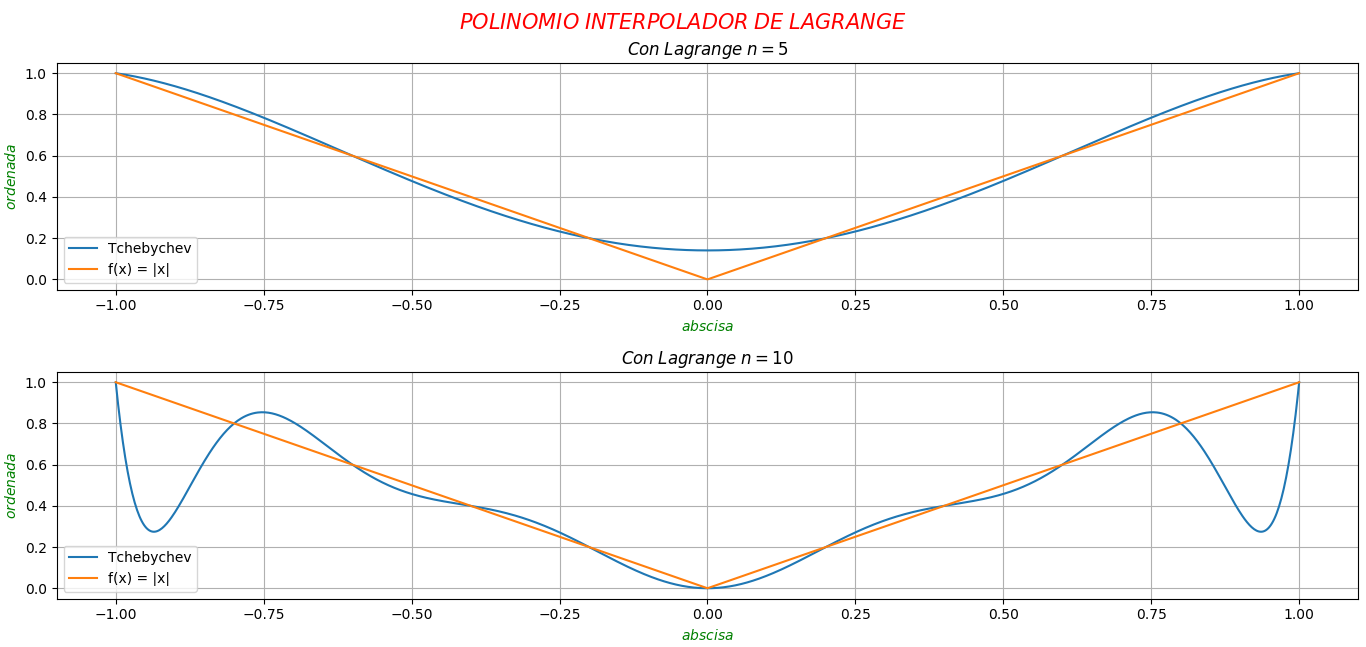
\includegraphics[width=8cm,height=5cm]{lagrange.png}
    \caption{Aproximación Lagrange con función módulo}
    \label{fig:modulo}
\end{figure}
Como se aprecia en la imagen para $n=10$, que es una cantidad baja, el problema se vuelve inestable. Te animo a que cambies en el código el valor de $n$ para que veas que al aumentar su valor el problema es cada vez más inestable. Para solucionar esto primero definiremos los polinomios de Tchebychev.
\section{Polinomios De Tchebychev}
\subsection*{Definición}
Se definen los polinomios de Tchebychev como una sucesión infinita de polinomios $\{T_n\}_{n=0}^\infty$ dada de forma recurrente como:
$$
T_0(x)=1,\quad T_1(x)=x,\quad T_{n+1}(x)=2xT_n(x)-T_{n-1}(x);\,\,\forall\,n\in\mathbb{N}
$$
Veamos sus propiedades más importantes:
\subsection*{Propiedades}
\begin{enumerate}
    \item $T_n$ es un polinomio de grado $n$ con coeficiente director $2^{n-1},\,n\in\mathbb{N}$.
    \item $T_n(x)=\cos (n\cdot\arccos (x));\,x\in [-1,1],\,n\in\mathbb{N}\cup\{0\}$.
    \item $\forall\,n\in\mathbb{N}$ las $n$ raíces de $T_n$ en $[-1,1]$ son: $x_k=\cos \left( \dfrac{(2k+1)\pi}{2n} \right);\,0\leq k\leq n-1$.
    \item $T_n(x)=2^{n-1}\prod\limits_{k=0}^{n-1} \left( x-\cos \dfrac{(2k+1)\pi}{2n} \right)$.
    \item $T_n(x)=\sum\limits_{k=0}^{\left[\frac{n}{2}\right]}\binom{n}{2k}x^{n-2k}\cdot (x^2-1)^k$.
    \item $T_{2n}$ es una función par, cuyo término independiente es $(-1)^n$. $T_{2n-1}$ es una función impar, sin término independiente.
    \item Los polinomios de Tchebychev forman una \textbf{base ortogonal de polinomios} en $[-1,1]$, con \textbf{función peso} es $\omega (x)=\dfrac{1}{\sqrt{1-x^2}}$.
\end{enumerate}
\subsection*{Notación}
Vamos a denotar el conjunto de polinomios mónicos de grado $n\in\mathbb{N}\cup\{0\}$ con la expresión:
$$
\mathcal{P}_n^m=\{ P(x)=x^n+a_{n-1}x^{n-1}+\cdots +a_1x+a_0\in\mathcal{P}_n \}
$$
\subsection*{Teorema}
Sea $f\in\mathcal{C}^{n+1}([-1,1])$, la menor cota del error en la norma del máximo en la interpolación de $f$ se obtiene cuando se toma como abscisas de interpolación las $n+1$-raíces de Tchebychev, $x_k=\cos \dfrac{(2k+1)\pi}{2(n+1)};\,0\leq k\leq n$. Además:
$$
||E_n||_{L^\infty([-1,1])}=||f-P_n||_{L^\infty([-1,1])}\leq\dfrac{1}{2^n(n+1)!}||f^{(n+1)}||_{L^\infty([-1,1])}
$$
Para el caso de un intervalo $[a,b]$ cualquiera se tiene: $x_k=\dfrac{a+b}{2}+\dfrac{b-a}{2}\cos \dfrac{(2k+1)\pi}{2(n+1)};\,0\leq k\leq n$. Con cota de error:
$$
||E_n||_{L^\infty([a,b])}=||f-P_n||_{L^\infty([a,b])}\leq\dfrac{(b-a)^{n+1}}{2^{2n+1}(n+1)!}||f^{(n+1)}||_{L^\infty([a,b])}
$$
\subsubsection*{Nota}
Este teorema nos da la solución al ejemplo de la función valor absoluto, tomaremos como partición en las abscisas las raíces del teorema.
\subsection*{Ejemplo}
Calcular el polinomio interpolador de la función $f(x)=|x|$ en el intervalo $[-1,1]$ utilizando las raíces de los polinomios de Tchebychev.\newpage
\subsubsection*{Solución}
Para resolverlo crearemos un programa con Python, en el cual calcularemos la partición de las abscisas utilizando las raíces de los polinomios de Tchebychev, con esta partición calcularemos su polinomio de Lagrange. Esto lo compararemos con la función $f(x)=|x|$. Consideraremos los casos $n=5,10,20$, con sus respectivas gráficas.
\begin{lstlisting}[frame=none]
import numpy as np
from scipy.interpolate import lagrange
from numpy.polynomial.polynomial import Polynomial, polyval
import matplotlib.pyplot as plt


def tchebychev(n):
    x = np.empty(n + 1)
    for k in np.arange(0, n + 1):
        x[k] = np.cos(((2 * k +1) * np.pi) / (2 * (n + 1)))
    return x

f = lambda x: polyval(x, coefs[::-1])

def my_lagrange(n):
    x = tchebychev(n)
    y = np.empty(shape=n + 1, dtype=float)
    for i in np.arange(n + 1):
        y[i] = np.abs(x[i])
    poly = lagrange(x, y)
    coefs = Polynomial(poly).coef
    return coefs

def my_plot(n, subplots):
    global coefs
    partition = np.linspace(-1, 1, 1000)
    fig, axs = plt.subplots(subplots, sharey=True, constrained_layout=True)
    fig.canvas.set_window_title('Lagrange con Tchebychev')
    plt.suptitle(r'$POLINOMIO\; LAGRANGE\; CON\; TCHEBYCHEV$', fontsize=15, color='r')
    for j in np.arange(len(n)):
        coefs = my_lagrange(n[j])
        axs[j].set_title(r'$Con\; Tchebychev\; n = {0}$'.format(n[j]))
        axs[j].set_xlabel(r'$abscisa$', color='g')
        axs[j].set_ylabel(r'$ordenada$', color='g')
        axs[j].plot(partition, f(partition), partition, np.abs(partition))
        axs[j].grid(True)
        axs[j].legend(['Tchebychev', 'f(x) = |x|'], loc='best')
    plt.show()

if __name__ == "__main__":
    coefs = None
    my_plot((5, 10, 20), 3)
\end{lstlisting}
Con este código la solución la puedes apreciar en la siguiente imagen:
\begin{figure}[h!]
    \centering
    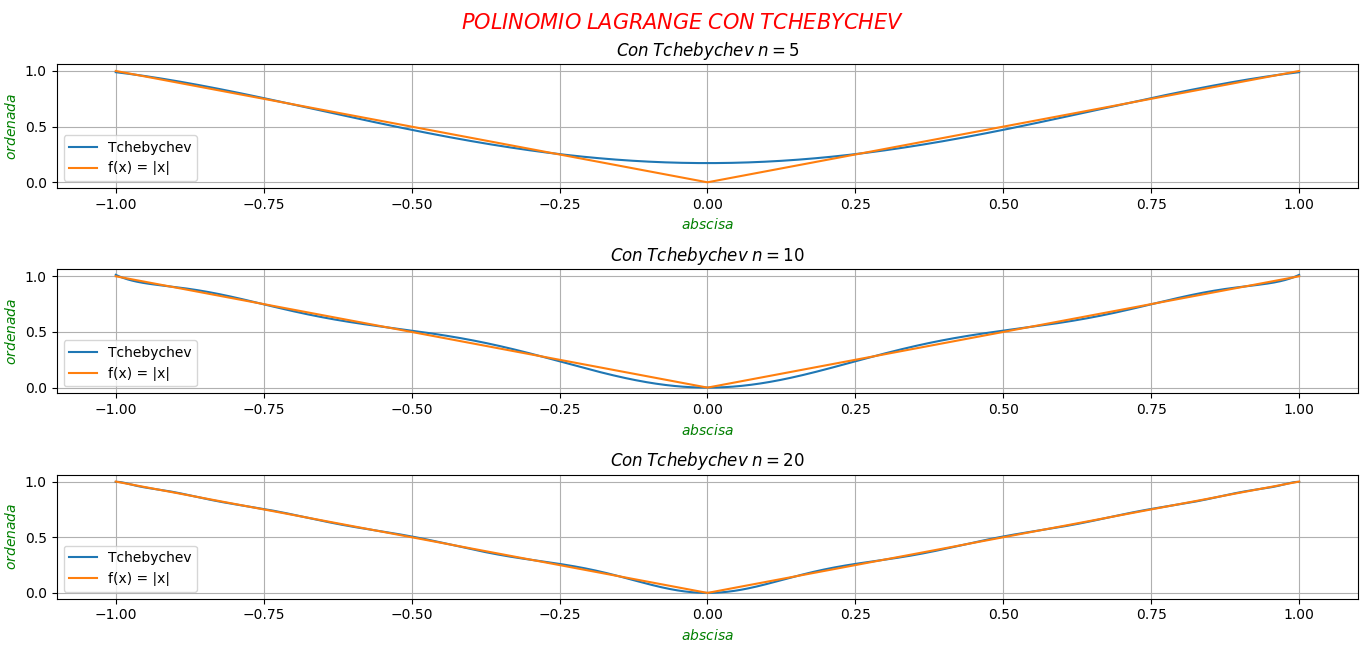
\includegraphics[width=8cm,height=5cm]{Lagrange_con_Tchebychev.png}
    \caption{Aproximación Lagrange con función módulo y Tchebychev}
    \label{fig:tchebychev}
\end{figure}
Vemos, que a diferencia del ejemplo anterior sin Tchebychev, al ir aumentando el tamaño de la partición nuestro polinomio interpolador de Lagrange se aproxima cada vez más a $f(x)=|x|$, de esa forma eliminamos la inestabilidad del ejemplo anterior.
\section{Interpolación De Newton}
Recordemos que utilizar Lagrange no es óptimo desde el punto de vista computacional por su alto coste, además si queremos añadir un nuevo nodo tendremos que volver a calcularlo todo desde el principio.
Estos dos inconvenientes pueden evitarse mediante el polinomio interpolador de Newton. Pero antes necesitaremos definir qué son las diferencias divididas.
\subsection*{Definición}
Consideremos $f:\;[a,\;b]\longrightarrow\;\mathbb{R}$, y una partición de nodos $\{ x_0,\cdots ,x_n \}\subset [a,\;b]$, distintos dos a dos. Denotemos $f(x_i)=f[x_i],\;0\leq i\leq n$. Definimos la \textbf{diferencia dividida de orden m} a la expresión:
$$
f[x_i,x_{i+1},\cdots ,x_{i+m}]=\dfrac{f[x_i,x_{i+1},\cdots ,x_{i+m-1}]-f[x_{i+1},x_{i+2},\cdots ,x_{i+m}]}{x_i-x_{i+m}}\;0\leq i\leq n;\;\forall\; m\in \mathbb{N}\cup\{0\}
$$
Notar que $f(x_i)=f[x_i],\;0\leq i\leq n$ es la diferencia dividida de orden 0 en el nodo $x_i$.
Definimos la \textbf{Diferencia finita de orden} $m\in \mathbb{N}\cup\{0\}$ de $f$ en $x_i$ como:
$$
\Delta^0f(x_i)=f(x_i);\;\Delta^mf(x_i)=\Delta^{m-1}f(x_{i+1})-\Delta^{m-1}f(x_i)
$$
Es fácil demostrar que $\Delta^m$ es un operador lineal.
\subsection*{Ejemplo}
Calcular las diferencias finitas y divididas de orden 2.
\subsubsection*{Solución}
$\Delta^2f(x_i)=\Delta f(x_{i+1})-\Delta f(x_i)=f(x_{i+2})-f(x_{i+1})-\left( f(x_{i+1})-f(x_i) \right)=\\=f(x_{i+2})-2f(x_{i+1})+f(x_i)$\\ \\
$f[x_i,x_{i+1},x_{i+2}]=\dfrac{f[x_i,x_{i+1}-f[x_{i+1},x_{i+2}]}{x_i-x_{i+2}}=\dfrac{1}{x_i-x_{i+2}}\left( \dfrac{f(x_i)-f(x_{i+1})}{x_i-x_{i+1}}-\dfrac{f(x_{i+1})-f(x_{i+2})}{x_{i+1}-x_{i+2}} \right)$

\subsection*{Teorema}
Sea $f:\;[a,\;b]\longrightarrow\;\mathbb{R}$, y una partición de nodos $\{ x_0,\cdots ,x_n \}\subset [a,\;b]$, distintos dos a dos. Consideremos $x_i=x_0+i\cdot h;\;h\in\mathbb{R}^{++},\;0\leq i\leq n$ (Equiespaciados). Se cumple:
$$
f[x_i,x_{i+1},\cdots ,x_{i+m}]=\dfrac{\Delta^mf(x_i)}{m!\cdot h^m}
$$
Si los nodos no son equiespaciados se cumple:
$$
f[x_i,x_{i+1},\cdots ,x_{i+m}]=\sum\limits_{j=0}^i \dfrac{f(x_j)}{\prod\limits_{k=0,k\neq j}^i (x_j-x_k)}\;0\leq i\leq n
$$
\subsection*{Corolario}
Sea $\sigma$ permutación de $\{0,1,\cdots ,i\}\rightarrow f[x_0,x_1,\cdots ,x_i]=f[x_{\sigma (0)},x_{\sigma (1)},\cdots ,x_{\sigma (i)}]$\\
Es decir; si reordenamos los nodos de la partición, el valor de la diferencia dividida se mantiene.\\ \\
Veamos mediante un teorema cuál es la fórmula de interpolación de Newton y su error:
\subsection*{Teorema (Fórmula Interpolación De Newton)}
Sea $f:[a,\; b]\longrightarrow\mathbb{R};\;\{ x_0,\cdots ,x_n\}\subset [a,\; b];\; x_i\neq x_j,\;i\neq j$. Se cumple:\\
$
P_n(x)=f(x_0)+\sum\limits_{i=1}^n \prod_{i-1}(x)f[x_0,\cdots ,x_i]=\\
=f(x_0)+(x-x_0)f[x_0,\;x_1]+(x-x_0)(x-x_1)f[x_0,\; x_1,\; x_2]+\cdots +(x-x_0)\cdot\cdots\cdot\\\cdot\cdots\cdot (x-x_{n-1})f[x_0,\;x_1,\cdots ,x_n]
$\\
$P_n(x)$ recibe el nombre de \textbf{Polinomio Interpolador De Newton De Grado n}. Con error:\\
$
E_n(x)=f(x)-P_n(x)=\prod_n (x)f[x_0,\;x_1,\cdots , x_n,\; x]\,/\,x\notin \{ x_0,\;x_1,\cdots ,x_n \}
$\\ \\
Además, $\exists\;\psi_x\in I_x\,/\, f[x_0,\cdots ,x_n,\; x]=\dfrac{f^{(n+1)}(\psi_x)}{(n+1)!}$\\ \\
Si $x_i = x_0 + i\cdot h\longrightarrow P_n(x)=f(x_0)+\sum\limits _{i=1}^n \prod_{i-1} (x)\dfrac{\Delta^i f(x_0)}{i!\cdot h^i}$.\\
Esta es la fórmula del polinomio interpolador de Newton de grado $n$ cuando los nodos están igualmente espaciados.
\subsection*{Nota}
El siguiente Corolario nos dice qué ocurre con el polinomio interpolador de Newton si añadimos un nodo más a la partición. Obviamente, al añadir un nodo el grado del polinomio aumenta en uno más.\newpage
\subsection*{Corolario}
Sea $x_{n+1}\in [a,\; b],\; x_{n+1}\notin \{x_0,\cdots ,x_{n+1} \}$, se cumple:\\ \\
$
P_{n+1}(x) = P_n(x) + \prod_n (x)f[x_0,\cdots ,x_{n+1}]
$\\ \\
En la fórmula se aprecia que añadir un nodo más es calcular sólo el siguiente término del polinomio interpolador; esto soluciona el segundo inconveniente que tiene el polinomio interpolador de Lagrange.
\subsection*{Ejemplo}
Dada la función $f(x)=\cos (\pi x)$, hallar el polinomio interpolador de Newton que interpola a $f$ en los puntos $\{ 0,\;0.5,\; 1,\; 1.5 \}$
\subsubsection*{Solución}
Lo vamos a resolver a mano para entender todos los conceptos, por esa razón hay pocos nodos en la partición. Como tenemos $4$ nodos, el grado del polinomio va a ser menor o igual a 3. Lo primero que debemos hacer es calcular las imágenes de los nodos mediante la función. Te dejo a ti los cálculos, te pongo la tabla.\\ \\
\begin{center}
    \begin{tabular}{|c||c|c|c|c|}
        \hline
        $x_i$ & 0 & 0.5 & 1 & 1.5 \\ \hline
        $f(x_i)$ & 1 & 0 & -1 & 0 \\ \hline
    \end{tabular}
\end{center}
Date cuenta que los nodos son equiespaciados con distancia común $h=0.5$. Las diferencias divididas calculadas a mano son sencillas si lo hacemos con una tabla. Te pongo primero la tabla:
\begin{center}
    \begin{tabular}{|llll|}
        \hline
        \color{blue}{$f(x_0)=1$} & \color{blue}{$\Delta f(x_0)=-1$} & \color{blue}{$\Delta^2 f(x_0)=0$} & \color{blue}{$\Delta^3 f(x_0)=2$} \\
        $f(x_1)=0$ & $\Delta f(x_1)=-1$ & $\Delta^2 f(x_1)=2$ & \\
        $f(x_2)=-1$ & $\Delta f(x_2)=1$ & & \\ 
        $f(x_3)=0$ & & & \\ \hline
    \end{tabular}
\end{center}\newpage
Fíjate que el elemento (1, 2) de la tabla se obtiene restando (2, 1) - (1, 1) y así sucesivamente. De la tabla, para calcular el polinomio nos quedamos con los elementos de la primera fila de la tabla, pasemos a calcularlo:\\ \\
$
P(x)=f(x_0)+(x-x_0)\dfrac{\Delta f(x_0)}{h}+(x-x_0)(x-x_1)\dfrac{\Delta^2 f(x_0)}{2!\;h^2}+(x-x_0)(x-x_1)(x-x_2)\dfrac{\Delta^3 f(x_0)}{3!\;h^3}=\\ \\=1+x\cdot \dfrac{-1}{0.5}+x(x-0.5)\dfrac{0}{2!\cdot 0.5^2}+x(x-0.5)(x-1)\dfrac{2}{3!\cdot 0.5^3}
$\\ \\
Desarrollando y simplificando términos obtenemos que el polinomio interpolador de Newton es:
$$
\color{blue}{P(x)=\frac{8}{3}x^3-4x^2-\frac{2}{3}x+1}
$$
Notar que para calcular el polinomio interpolador de Newton hemos utilizado la expresión cuando los nodos son equiespaciados, como es el caso de este ejemplo.
\subsection*{Ejemplo}
Calcular el polinomio interpolador de Newton de la siguiente tabla de valores:
\begin{center}
    \begin{tabular}{|c||c|c|c|c|c|c|}
        \hline
        $x_i$ & 0.15 & 2.3 & 3.15 & 4.85 & 6.25 & 7.95 \\ \hline
        $f(x_i)$ &  4.79867 & 4.49013 & 4.2243 & 3.47313 & 2.66674 & 1.51909 \\ \hline
    \end{tabular}
\end{center}
\subsubsection*{Solución}
Obviamente este ejemplo tiene ya demasiados datos para hacerlo a mano, así que lo mejor es escribir un programa; lo haremos con Python, utilizando las librerías Numpy, Sympy y Matplotlib. El código es el siguiente:
\begin{lstlisting}[frame=none]
#/usr/bin/env python3
# -*- coding: utf-8 -*-


import numpy as np
from sympy import symbols, init_printing, lambdify, horner, expand, pprint
import matplotlib.pyplot as plt


x = symbols('x')
init_printing(use_unicode=True)


def diferencias(x, y, n):
    T = y
    for k in np.arange(1, n + 1):
        T[k: n] = (T[k: n] - T[k - 1]) / (x[k: n] - x[k - 1])
    return T


def polnewtonsym(diff, xx):
    n = len(xx) - 1
    pol = diff[n]
    for k in np.arange(1, n + 1):
        pol = diff[n - k] + (x - xx[n - k])*pol
    return pol


datosx = np.array([0.15, 2.3, 3.15, 4.85, 6.25, 7.95], dtype=float)
datosy = np.array([4.79867, 4.49013, 4.2243, 3.47313, 2.66674, 1.51909], dtype=float)
datosy2 = datosy.copy()
diff = diferencias(datosx, datosy, len(datosx))
polnewtonsym = polnewtonsym(diff, datosx)
pprint('El polinomio interpolador de Newton es:')
pprint(expand(polnewtonsym))
polnewtonsym = horner(polnewtonsym)
P = lambdify(x, polnewtonsym, 'numpy')
t = np.linspace(datosx[0], datosx[-1], 1000)

plt.axis([0.0, 8.0, -2.0, 5.0])
plt.grid(True)
plt.suptitle(r'$ALGORITMO\; POLINOMIO\; INTERPOLADOR\; DE\; NEWTON.$', fontsize=20, color='r')
title = r'$Polinomio \; Interpolador \; Newton \; Grado \; n={}$'.format(len(datosx) - 1)
plt.title(title, fontsize=18, color='b')
plt.xlabel(r'$Datos\; x$', color='blue', fontsize=20)
plt.ylabel(r'$Datos\; y$', color='blue', fontsize=20)
plt.scatter(datosx, datosy2, c='r', s=70, edgecolors='r')
plt.plot(t, P(t), 'b-', lw=1.5)

text1 = r'$Pol.\; Newton$'
text2 = r'$Puntos\; Tabla$'
legend = plt.legend([text1, text2], scatterpoints=1, markerscale = 1.5, shadow=True, loc='best')
frame = legend.get_frame()
frame.set_facecolor('0.90')

xtcks = np.arange(0, 9)
xtckslatex = []
for i in xtcks:
    xtckslatex.append('$' + str(i) + '$' )
ytcks = np.arange(-2, 6)
ytckslatex = []
for i in ytcks:
    ytckslatex.append('$' + str(i) + '$' )
plt.xticks(xtcks, xtckslatex, fontsize=18)
plt.yticks(ytcks, ytckslatex, fontsize=18)

plt.show()
\end{lstlisting}
Te dejo a ti que ejecutes y experimentes con el código y la solución del ejemplo, no tiene mucho misterio.
\section{Método De Neville}
Este método de interpolación resuelve la dificultad de los polinomios Lagrange en los que el término del error es difícil de aplicar, ya que el grado del polinomio que se necesita para la aproximación deseada es generalmente no conocido. Resolveremos el inconveniente aprovechando los cálculos de los pasos anteriores.
\subsection*{Definición}
Sea $f$ una función definida en los nodos $x_0,\,\dots ,x_n$. Consideremos $m_1,\dots ,m_k\,\in\,\mathbb{Z}$ distintos con $0\leq m_i\leq n,\,\forall\, i$. El polinomio Lagrange que coincide con $f(x)$ en $x_{m_1},\dots ,x_{m_k}$ se denota como $P_{m_1,\, m_2,\dots ,\, m_k}(x)$.\\
Veamos un teorema con el cual se describe un método para generar recursivamente aproximaciones polinómicas de Lagrange.
\subsection*{Teorema (Método Neville)}
Sea $f$ una función definida en los nodos $x_0,\,\dots ,x_n\,/\, x_i\neq x_j;\,i\neq j;\, 0\leq i,\, j\leq k \longrightarrow $ Se cumple que el k-ésimo polinomio Lagrange que interpola la función en dichos nodos viene determinado como:
\[
P(x)=\dfrac{(x-x_j)P_{0,\,1,\dots ,j-1,\,j+1,\dots ,\, k}(x)-(x-x_i)P_{0,\,1,\dots ,i-1,\,i+1,\dots ,\, k}(x) }{(x_i-x_j)}
\]
\subsection*{Notación}
Para evitar múltiples subíndices tomamos el polinomio interpolación de grado $j$ en los $j+1$ nodos $x_{i-j},\, x_{i-j+1},\dots ,x_{i-1},\, x_i$ por $Q_{i,\, j}(x)$, es decir;
\[
Q_{i,\, j} = P_{i-j,\, i-j+1,\,\dots ,i-1,\, i}
\]
\subsection*{Código Neville}
Te dejo el código del algoritmo Neville con un pequeño ejemplo aplicado.
\begin{lstlisting}[frame=none]
#/usr/bin/env python3
# -*- coding: utf-8 -*-

import numpy as np

def neville(x, y, x0):
    n = len(x)
    Q = np.zeros(shape=(n, n), dtype=float)
    for i in np.arange(n):
        Q[i][0] = y[i]
    for i in np.arange(1, n):
        for j in np.arange(1, i + 1):
            f = (x0-x[i-j]) * Q[i][j - 1] - (x0 - x[i]) * Q[i - 1][j - 1]
            g = x[i] - x[i -j]
            Q[i][j] = f / g
    print(Q)

if __name__ == '__main__':
    x = np.array([1.0, 1.3, 1.6, 1.9, 2.2], dtype=float)
    y = np.array([0.7651977, 0.6200860, 0.4554022, 0.2818186, 0.1103623])
    neville(x, y, 1.5)
\end{lstlisting}

\section{Interpolación Hermite}
Otro tipo de interpolación polinómica se basa en los polinomios de interpolación de Hermite, y que algorítmicamente hablando los implementaremos utilizando las diferencias divididas.
\subsection*{Definición}
Sea $f\in\mathcal{C}^1([a,\;b])$, consideremos los nodos $x_0,\;\dots\;,x_n\in [a,\;b],\,x_i\neq x_j\rightarrow\;\exists\;!\;$ polinomio en el conjunto de nodos dado, llamado \textbf{Polinomio De Hermite}, de grado al menos $2n+1$ dado por:
\[
H_{2n+1}(x)=\sum\limits_{j=0}^n f(x_j)H_{n,\; j}(x)+\sum\limits_{j=0}^n f^\prime (x_j)\hat{H}_{n,\; j}(x)
\]
con $H_{n,\; j}(x)=[1-2(x-x_j)]L^\prime _{n,\; j}(x_j)L^2_{n,\; j}(x),\,\hat{H}_{n,\; j}(x)=(x-x_j)L^2_{n,\; j}(x)$.\\ \\
Si $f\in\mathcal{C}^{2n+2}([a,\;b])\rightarrow\;\exists\;\psi_x\in ]a,\;b[\;$ tal que:
\[
f(x)=H_{2n+1}(x)+\dfrac{(x-x_0)^2\cdots (x-x_n)^2}{(2n+2)!}f^{(2n+2)}(\psi_x)
\]
\subsection*{Ejemplo}
Dada la siguiente tabla de valores de una función, calcula aproximadamente $f(1.5)$ utilizando Hermite.
\begin{center}
    \begin{tabular}{|c||c|c|c|}
        \hline
        $k$  & $x_k$ & $f(x_k)$  & $f^\prime (x_k)$\\ \hline
        0    & 1.3   & 0.6200860 & -0.5220232 \\ \hline
        1    & 1.6   & 0.4554022 & -0.5698959 \\ \hline
        2    & 1.9   & 0.2818186 & -0.5811571 \\ \hline
    \end{tabular}
\end{center}
\subsubsection*{Solución}
Tenemos que $n=2$. Primero calculamos los polinomios Lagrange y sus derivadas.
\begin{center}
    \begin{tabular}{ll}
        $L_{2,\;0}(x)=\dfrac{(x-x_1)(x-x_2)}{(x_0-x_1)(x_0-x_2)}=\frac{50}{9}x^2-\frac{175}{9}x+\frac{152}{9}$    & $L^\prime _{2,\;0}(x)=\frac{100}{9}x-\frac{175}{9}$ \\
        $L_{2,\;1}(x)=\dfrac{(x-x_0)(x-x_2)}{(x_1-x_0)(x_1-x_2)}=\frac{-100}{9}x^2+\frac{320}{9}x-\frac{247}{9}$    & $L^\prime _{2,\;1}(x)=\frac{-200}{9}x-\frac{320}{9}$ \\
        $L_{2,\;2}(x)=\dfrac{(x-x_0)(x-x_1)}{(x_2-x_0)(x_2-x_1)}=\frac{50}{9}x^2-\frac{145}{9}x+\frac{104}{9}$    & $L^\prime _{2,\;2}(x)=\frac{100}{9}x-\frac{145}{9}$
    \end{tabular}
\end{center}
Calculemos los polinomios asociados al polinomio de Hermite:
\[
H_{2,\;0}(x)=[1-2(x-1.3)(-5)]\left( \frac{50}{9}x^2-\frac{175}{9}x+\frac{152}{9} \right)^2=(10x-12)\left( \frac{50}{9}x^2-\frac{175}{9}x+\frac{152}{9} \right)^2
\]
\[
H_{2,\;1}(x)=[1-2(x-1.6)\left(-\frac{200}{9}1.6+\frac{320}{9}\right)]\left( \frac{-100}{9}x^2+\frac{320}{9}x-\frac{247}{9} \right)^2=\left( \frac{-100}{9}x^2+\frac{320}{9}x-\frac{247}{9} \right)^2
\]
\[
H_{2,\;2}(x)=10(2-x)\left( \frac{50}{9}x^2-\frac{145}{9}x+\frac{104}{9} \right)^2\quad \hat{H}_{2,\;0}(x)=(x-1.3)\left( \frac{50}{9}x^2-\frac{175}{9}x+\frac{152}{9} \right)^2
\]
\[
\hat{H}_{2,\;1}(x)=(x-1.6)\left( \frac{-100}{9}x^2+\frac{320}{9}x-\frac{247}{9} \right)^2\quad \hat{H}_{2,\;2}(x)=(x-1.9)\left( \frac{50}{9}x^2-\frac{145}{9}x+\frac{104}{9} \right)^2
\]
Con todos estos polinomios los sustituimos y obtenemos como polinomio interpolador de Hermite:
\[
H_5(x)=0.6200860H_{2,\;0}(x)+0.4554022H_{2,\;1}(x)+0.2818186H_{2,\;2}(x)-0.5220232\hat{H}_{2,\;0}(x)-
\]
\[
-0.5698939\hat{H}_{2,\;1}(x)-0.5811571\hat{H}_{2,\; 2}(x)
\]
Si sustituimos en el polinomio anterior $x=1.5$ obtenemos como solución aproximada $$f(1.5)\approx H(1.5)=0.5118277$$
Como puedes ver en este ejemplo hay que hacer una ingente cantidad de cálculos, pero además; estamos utilizando los polinomios de Lagrange, los cuales ya sabemos no son óptimos. Todos estos obstáculos los evitamos redefiniendo el polinomio interpolador de Hermite utilizando el concepto de diferencia dividida.
\subsection*{Polinomios De Hermite Utilizando Diferencias Divididas}
Consideremos $P_n(x)=f[x_0]+\sum\limits_{k=1}^n f[x_0,\dots ,x_k](x-x_0)\cdots (x-x_{k-1})$\\
Definimos una sucesión de nodos ${z_i}_{i=0}^{2n+1}$ por $z_{2i}=z_{2i+1}=x_i,\;0\leq i\leq n$. De esa forma vamos a poder utilizar de la tabla las derivadas.\\
Tenemos que: $f[z_{2i},\;z_{2i+1}]=f^\prime (z_{2i})=f^\prime (x_i)$, de esa forma podemos utilizar las entradas:\\ $f^\prime (x_0),\dots ,f^\prime (x_n)$ en vez de $f[z_0,\;z_1],\;f[z_2,\;z_3],\dots ,f[z_{2n},\;z_{2n+1}]$.\\
Con todo esto redefinimos el polinomio interpolador de Hermite de grado $2n+1$, utilizando diferencias divididas, como:
\[
H_{2n+1}(x)=f[z_0]+\sum\limits_{k=1}^{2n+1}f[z_0,\dots ,z_k](x-z_0)\cdots (x-z_{k-1})
\]\newpage
\subsection*{Ejemplo}
Volver a calcular $f(1.5)$ del ejemplo anterior pero utilizando el polinomio interpolador de Hermite con diferencias divididas.
\subsubsection*{Solución}
\begin{center}
    \begin{tabular}{|l||llllll|}
        \hline
        $1.3$ & \color{blue}{$0.6200860$} & & & & & \\
          & & \color{blue}{$-0.5220232$} & & & & \\
        $1.3$ & $0.6200860$ & & \color{blue}{$-0.0897427$} & & & \\
          & & $-0.5489460$ & & \color{blue}{$0.0663657$} & & \\
        $1.6$ & $0.4554022$ & & $-0.0698330$ & & \color{blue}{$0.0026663$} & \\
        & & $-0.5698959$ & & $0.0679655$ & & \color{blue}{$-0.0027738$}\\
        $1.6$ & $0.4554022$ & & $-0.0290537$ & & $0.0010020$ & \\
        & & $-0.5786120$ & & $0.0685667$ & &  \\
        $1.9$ & $0.2818186$ & & $-0.0084837$ & & & \\
        & & $-0.5811571$ & & & & \\
        $1.9$ & $0.2918186$ & & & & & \\ \hline
    \end{tabular}
\end{center}
En la tabla de las diferencias divididas nos quedamos con las que están coloreadas de azul.\\
Tenemos pues la solución:\\
$H_5(1.5)=f[1.3]+f[1.3](1.5-1.3)+f[1.3,\;1.3,\;1.6](1.5-1.3)^2+f[1.3,\;1.3,\;1.6,\;1.6](1.5-1.3)^2(1.5-1.6)+f[1.3,\;1.3,\;1.6,\;1.6,\;1.9](1.5-1.3)^2(1.5-1.6)^2+f[1.3,\;1.3,\;1.6,\;1.6,\;1.9,\;1.9](1.5-1.3)^2(1.5-1.6)^2(1.5-1.9)\approx \color{blue}{0.5118277}$
\subsection*{Algoritmo Polinomio Interpolador De Hermite}
Veamos el código del polinomio interpolador de Hermite utilizando diferencias divididas. El código viene aplicado con el ejemplo anterior para que puedas practicar:
\begin{lstlisting}[frame=none]
#/usr/bin/env python3
# -*- coding: utf-8 -*-


import numpy as np
from sympy import symbols, init_printing, lambdify, horner, expand, pprint
import matplotlib.pyplot as plt


x = symbols('x')
init_printing(use_unicode=True)


def diferencia(x, y, yp):
    n = len(x)
    z = np.empty(shape=2 * n, dtype=float)
    Q = np.zeros(shape=(2 * n, 2 * n), dtype=float)
    d = np.empty(shape=2 * n, dtype=float)

    for i in np.arange(n):
        z[2 * i] = x[i]
        z[2 * i + 1] = x[i]
        Q[2 * i][0] = y[i]
        Q[2 * i + 1][0] = y[i]
        Q[2 * i + 1][1] = yp[i]
        if i !=0:
            Q[2 * i][1] = (Q[2 * i][0] - Q[2 * i - 1][0]) / (z[2 * i] - z[2 * i - 1])

    for i in np.arange(2, 2 * (n - 1) + 2):
        for j in np.arange(2, i + 1):
            f = Q[i][j - 1] - Q[i - 1][j - 1]
            g = z[i] - z[i - j]
            Q[i][j] = f / g
    d = Q.diagonal()
    return z, d

def polhermitesym(diff, z):
    n = len(z) - 1
    pol = diff[n]
    for k in np.arange(1, n + 1):
        pol = diff[n - k] + (x - z[n - k])*pol
    return pol

if __name__ == '__main__':    
    datos_x = np.array([1.3, 1.6, 1.9], dtype=float)
    datos_y = np.array([0.6200860, 0.4554022, 0.2818186], dtype=float)
    datos_yp = [-0.5220232, -0.5698959, -0.5811571]

    d = diferencia(datos_x, datos_y, datos_yp)
    diff = d[1]
    polhermitesym = polhermitesym(diff, d[0])
    pprint('El polinomio interpolador de Hermite es:')
    pprint(expand(polhermitesym))
    pprint('El valor aproximado obtenido con x={0} es H({0})={1}'.format(1.5, polhermitesym.subs(x, 1.5)))
\end{lstlisting}
Al ejecutarlo obtenemos como valor aproximado: $H(1.5)=0.511827701728395$, que como se puede apreciar es la misma aproximación que la anterior, pero con más decimales debido a la precisión del ordenador.\\
Con esto termina este apartado dedicado al polinomio interpolador de Hermite, el cual respecto al de Newton su gran diferencia es que también se utilizan los valores de la derivada de la función. Con esto, a priori podemos pensar que siempre obtendremos una mejor aproximación respecto al de Newton por utilizar los datos de la primera derivada aunque haya un mayor número de cálculos por utilizar un mayor número de datos entrada.
\section{Interpolación Spline}
Es un tipo de interpolación polinómica en el que dada una partición de nodos interpolamos con un polinomio cada dos nodos consecutivos. Veámoslo con mucho más detalle.
\subsection*{Definición}
Tomemos $\Delta = \{ a=x_0<x_1<\cdots <x_n=b \}$ partición de $[a,\;b]$ y $S_\Delta :[a,\;b]\longrightarrow\mathbb{R}$. Decimos que $S_\Delta$ es una \textbf{Función Spline De Orden k Asociada a } $\Delta$ si $S_\Delta \in\mathcal{C}^{k+1} ([a,\;b])$ y $S_\Delta$ coincide con un polinomio de grado $\leq k$ en cada intervalo $[x_i,\;x_{i+1}];\;0\leq i\leq n-1$.\\
Para $k=1$ tenemos que la función spline es una función lineal a trozos (una poligonal). Para $k=3$ la función spline se le llama \textbf{Función Spline Cúbica}, es la más utilizada con diferencia.\\
Para mejor comprensión de los splines aquí sólo lo veremos para el caso del spline cúbico.\\
Sea $y=(y_0,\cdots ,\; y_n)\in\mathbb{R}^{n+1}\longrightarrow\;S_\Delta (y,\;\cdot )$ será una función spline cúbica de interpolación que verificará: $S_\Delta (y,\; x_i)=y_i;\; 0\leq i\leq n$.
\subsection*{Observación}
Sea $y=(y_0,\; y_1,\; y_2,\; y_3)\in\mathbb{R}^4$, con función spline $S_\Delta \in\mathcal{C}^2 ([x_0,\; x_3])$. La expresión general de la función spline es:
\[ S_\Delta (y,\; x) = \left\{ 
 \begin{array}{ll}
  a_3x^3+a_2x^2+a_1x+a_0; & x\in [x_0,\; x_1]\\
  b_3x^3+b_2x^2+b_1x+b_0; & x\in [x_1,\; x_2]\\
  c_3x^3+c_2x^2+c_1x+c_0; & x\in [x_2,\; x_3]
 \end{array} \right.
\]
Imponiendo las condiciones $S_\Delta (y,\;x_i)=y_i;\;i=0,\;1,\;2,\;3$ tenemos el sistema:
\[
\left\{ 
 \begin{array}{lcl}
  a_3x_0^3+a_2x_0^2+a_1x_0+a_0 & = & y_0\\
  a_3x_1^3+a_2x_1^2+a_1x_1+a_0 & = & y_1\\
  b_3x_1^3+b_2x_1^2+b_1x_1+b_0; & = & y_1\\
  b_3x_2^3+b_2x_2^2+b_1x_2+b_0; & = & y_2\\
  c_3x_2^3+c_2x_2^2+c_1x_2+c_0; & = & y_2\\
  c_3x_3^3+c_2x_3^2+c_1x_3+c_0; & = & y_3
 \end{array} \right.
\]
Derivemos las ecuaciones anteriores y las igualamos 2 a 2 de forma alterna, obtenemos las ecuaciones:
\[
\left\{ 
 \begin{array}{lcl}
  3a_3x_1^2+2a_2x_1+a_1 & = & 3b_3x_1^2+2b_2x_1+b_1\\
  3b_3x_2^2+2b_2x_2+b_1; & = & 3c_3x_2^2+2c_2x_2+c_1
 \end{array} \right.
\]
Finalmente derivamos las 2 ecuaciones anteriores obteniendo:
\[
\left\{ 
 \begin{array}{lcl}
  6a_3x_1+2a_2 & = & 6b_3x_1+2b_2\\
  6b_3x_2+2b_2; & = & 6c_3x_2+2c_2
 \end{array} \right.
\]
Uniendo todas las ecuaciones (libres) tenemos un sistema de 10 ecuaciones con 12 incógnitas y $12-10=2$ grados de libertad.\\
En el caso general tenemos, $4n-2$ ecuaciones, $2n$ ecuaciones de los valores que interpola $S_\Delta$, $n-1$ ecuaciones son de la continuidad de $S_\Delta ^\prime$, y las restantes $n-1$ ecuaciones provienen de la continuidad de $S_\Delta ^{\prime\prime}$.\\
Con todas estas condiciones tenemos 3 tipos diferentes de funciones spline:\\
\textbf{TIPO I} $\longrightarrow S_\Delta ^{\prime\prime} (y,\; a)=S_\Delta ^{\prime\prime} (y,\; b)=0$. Se les denomina \textbf{Condiciones Naturales}.\\
\textbf{TIPO II} $\longrightarrow S_\Delta ^{\prime} (y,\; a)=y_0^\prime ,\; S_\Delta ^{\prime} (y,\; b)=y_n^\prime$ con $y_0^\prime ,\;y_n^\prime \in\mathbb{R}$ valores prefijados.\\
\textbf{TIPO III} $\longrightarrow S_\Delta ^{(k)} (y,\; a)=S_\Delta ^{(k)} (y,\; b);\;k=0,\;1,\;2$. Son para funciones periódicas de periodo $b-a$, es decir; $y_0=y_n$.
\subsection*{Método De Cálculo De Funciones Spline Cúbicas}
No voy a escribir todos los cálculos, voy a poner un resumen de todo los pasos a realizar en todos los tipos. Partimos de un sistema matricial $A\cdot M=d$, donde $M$ es la matriz de incógnitas. Para los tres casos tenemos los parámetros siguientes:
\[
h_{j+1}=x_{j+1}-x_j;\;0\leq j\leq n-1\quad \lambda_j=\dfrac{h_{j+1}}{h_j+h_{j+1}};\quad\mu_j=1-\lambda_j
\]
\[
d_j=\dfrac{6}{h_j+h_{j+1}}\left( \dfrac{y_{j+1}-y_j}{h_{j+1}}-\dfrac{y_j-y_{j-1}}{h_j} \right);\;1\leq j\leq n-1
\]
Si los nodos son equiespaciados tendremos:
\[
\lambda_i=\mu_i=\frac{1}{2};\quad d_i=3\cdot\dfrac{y_{i+1}-2y_i+y_{i-1}}{h^2};\;1\leq i\leq n-1
\]
\textbf{TIPO I}$\longrightarrow M_0=M_n=0;\; \lambda_0=d_0=\mu_n=d_n=0$\\
\textbf{TIPO II}$\longrightarrow \lambda_0=\mu_n=1;\;d_0=\frac{6}{h_2}\left( \dfrac{y_1-y_0}{h_1}-y_0^\prime \right);\;d_n=\frac{6}{h_n}\left( y_n^\prime - \dfrac{y_n-y_{n-1}}{h_n} \right)$\\
\textbf{TIPO III}$\longrightarrow M_0=M_n;\;\lambda_n=\dfrac{h_1}{h_1+h_n};\;\mu_n = 1-\lambda_n;\;d_n=\dfrac{6}{h_1+h_n}\left( \dfrac{y_1-y_n}{h_1}-\dfrac{y_n-y_{n-1}}{h_n} \right)$\\
En los tipos I y II las matrices del sistema tienen la estructura:
\[
A=
\begin{pmatrix}
    2 & \lambda_0 &        &         &\\
\mu_1 & 2      & \lambda_1 &         &\\
      & \mu_2  & 2         & \lambda_2  &\\
      & \ddots & \ddots    & \ddots & \\
      &        & \mu_{n-1} & 2      & \lambda_{n-1}\\
      &        &           & \mu_n  & 2
\end{pmatrix}\quad
M=
\begin{pmatrix}
    M_0\\
    M_1\\
    \vdots\\
    M_n
\end{pmatrix}\quad
d=
\begin{pmatrix}
    d_0\\
    d_1\\
    \vdots\\
    d_n
\end{pmatrix}
\]
Para el tipo III consideramos el sistema $A_p=M_p\cdot d_p$ con la forma:
\[
A_p=
\begin{pmatrix}
    2 & \lambda_1 &        &         & \mu_1\\
\mu_2 & 2      & \lambda_2 &         &\\
      & \mu_2  & 2         & \lambda_2  &\\
      & \ddots & \ddots    & \ddots & \\
      &        & \mu_{n-1} & 2      & \lambda_{n-1}\\
\lambda_n      &        &           & \mu_n  & 2
\end{pmatrix}\quad
M_p=
\begin{pmatrix}
    M_1\\
    M_2\\
    \vdots\\
    M_n
\end{pmatrix}\quad
d_p=
\begin{pmatrix}
    d_1\\
    d_2\\
    \vdots\\
    d_n
\end{pmatrix}
\]
Finalmente la expresión general de la función de spline para los tres tipos viene dada por:\\
$
S_\Delta (y,\; x)=y_j + \left( \dfrac{y_{j+1}-y_j}{h_{j+1}}-\dfrac{2M_j+M_{j+1}}{6}\cdot d_{j+1} \right)(x-x_j)+\frac{M_j}{2}(x-x_j)^2+\\ + \dfrac{M_{j+1}-M_j}{6h_{j+1}}(x-x_j)^3;\;x\in [x_j,\;x_{j+1}];\;0\leq j\leq n-1
$
\subsection*{Ejemplo}
Determinar la función spline cúbica que interpola los datos de la tabla:
\begin{center}
    \begin{tabular}{|c||c|c|c|}
        \hline
        $x_i$    & 0 & 1 & 3 \\ \hline
        $f(x_i)$ & 1 & 2 & 0 \\ \hline
    \end{tabular}
\end{center}
Por los datos de la tabla sabemos que es un spline cúbico de tipo I. Y por ser de tipo I tenemos:
$$
\lambda_0 = d_0 = \mu_2 = d_2 = 0
$$
Calculemos primero los $h_{j+1} = x_{j+1}-x_j\longrightarrow h_1=1-0=1;\; h_2=3-1=2$.\\
Los otros cálculos:\\ \\
$\lambda_1 = \dfrac{h_2}{h_1+h_2}=\frac{2}{1+2}=\frac{2}{3};\,\,\mu_1 = 1-\lambda_1=1-\frac{2}{3}=\frac{1}{3}$\\
$d_1=\dfrac{6}{h_1+h_2}\left( \dfrac{y_2-y_1}{h_2}-\dfrac{y_1-y_0}{h_1} \right)=\frac{6}{1+2}\left( \frac{0-2}{2}-\frac{2-1}{1} \right)=-4$\\ \\
Montamos la matriz de coeficientes:
\[
A=
\begin{pmatrix}
    2 & \lambda_0 & 0\\
\mu_1 & 2  & \lambda_1 \\
    0 & \mu_2  & 2
\end{pmatrix} =
\begin{pmatrix}
    2 & 0 & 0\\
 \frac{1}{3} & 2  & \frac{2}{3} \\
    0 & 0 & 2
\end{pmatrix}
\]
Con esto tenemos como sistema matricial:
\[
\begin{pmatrix}
    2 & 0 & 0\\
 \frac{1}{3} & 2  & \frac{2}{3} \\
    0 & 0 & 2
\end{pmatrix}\cdot
\begin{pmatrix}
    M_0\\ M_1 \\ M_2
\end{pmatrix}=
\begin{pmatrix}
    0\\ -4 \\ 0
\end{pmatrix}
\]
La solución del sistema es: $M_0=0,\;M_1=-2,\;M_2=0$. Haciendo los cálculos pertinentes obtienes como función spline:
\[ S_\Delta (y,\; x) = \left\{ 
 \begin{array}{ll}
  1+\frac{4}{3}x-\frac{1}{3}x^3; & x\in [0,\; 1]\\
  2+\frac{1}{3}(x-1)-(x-1)^2+\frac{1}{6}(x-1)^3; & x\in [1,\; 3]
 \end{array} \right\}
\]
\subsection*{Ejemplo}
Calcular la función spline cúbica de tipo III según la siguiente tabla de datos:
\begin{center}
    \begin{tabular}{|c||c|c|c|c|}
        \hline
        $x_i$    & -1 & 0 & 1 & 3 \\ \hline
        $f(x_i)$ & -4 & -1 & 0 & 20\\ \hline
        $f^\prime(x_i)$ & 6 &  &  & 22\\ \hline
    \end{tabular}
\end{center}
\subsubsection*{Solución}
Tenemos que: $h_1=1,\; h_2=1,\; h_3=2$. Además: $\lambda_0=\mu_3=1$, donde $n=3$. También, por ser de Tipo III tenemos los siguientes valores:
$$
d_0=\frac{6}{h_1}\left(\dfrac{y_1-y_0}{h_1}-y_0^\prime \right)=\frac{6}{1}\left( \dfrac{-1-(-4)}{1}-6 \right)\rightarrow d_0=-18
$$
$$
d_3=\frac{6}{h_3}\left( y_3^\prime -\dfrac{y_3-y_2}{h_3} \right)=\frac{6}{2}\left( 22-\dfrac{20-0}{2} \right)\rightarrow d_3=36
$$
Calculemos los d's restantes según la fórmula general:
$$
d_1=\frac{6}{h_1+h_2}\left( \dfrac{y_2-y_1}{h_2} -\dfrac{y_1-y_0}{h_1} \right)=\frac{6}{1+1}\left( \dfrac{0-(-1)}{1}-\dfrac{-1-(-4)}{1} \right)\rightarrow d_1=-6
$$
$$
d_2=\frac{6}{h_2+h_3}\left( \dfrac{y_3-y_2}{h_3} -\dfrac{y_2-y_1}{h_2} \right)=\frac{6}{1+2}\left( \dfrac{20-0}{2}-\dfrac{0-(-1)}{1} \right)\rightarrow d_1=18
$$
Ahora debemos calcular los lambdas y mus faltantes:
$$
\lambda_1=\dfrac{h_2}{h_1+h_2}=\dfrac{1}{1+1}\rightarrow \lambda_1=\frac{1}{2};\quad \mu_1=1-\frac{1}{2}\rightarrow\mu_1=\frac{1}{2}
$$
$$
\lambda_2=\dfrac{h_3}{h_2+h_3}=\dfrac{2}{1+2}\rightarrow \lambda_2=\frac{2}{3};\quad \mu_2=1-\frac{2}{3}\rightarrow\mu_1=\frac{1}{3}
$$
Reuniendo los cálculos tenemos que la matriz de coeficientes del sistema matricial $A\cdot M=d$ es:
\[
A=
\begin{pmatrix}
    2 & \lambda_0 & 0 & 0\\
\mu_1 & 2  & \lambda_1 & 0\\
    0 & \mu_2  & 2 & \lambda_2\\
    0 &   0    & \mu_3 & 2
\end{pmatrix} =
\begin{pmatrix}
    2 & 1 & 0 & 0\\
 \frac{1}{2} & 2 & \frac{1}{2} & 0\\
       0     & \frac{1}{3} & 2 & \frac{2}{3}\\
    0 & 0 & 1 & 2
\end{pmatrix}
\]
Así pues, el sistema matricial nos queda de la siguiente forma:
\[
\begin{pmatrix}
    2 & \lambda_0 & 0 & 0\\
\mu_1 & 2  & \lambda_1 & 0\\
    0 & \mu_2  & 2 & \lambda_2\\
    0 &   0    & \mu_3 & 2
\end{pmatrix} =
\begin{pmatrix}
    2 & 1 & 0 & 0\\
 \frac{1}{2} & 2 & \frac{1}{2} & 0\\
       0     & \frac{1}{3} & 2 & \frac{2}{3}\\
    0 & 0 & 1 & 2
\end{pmatrix}\cdot
\begin{pmatrix}
    M_0\\ M_1\\ M_2\\ M_3
\end{pmatrix}=
\begin{pmatrix}
    -18\\ -6\\ 18\\ 36
\end{pmatrix}
\]
Te dejo a ti que lo resuelvas, la solución es la siguiente:
\[
M_0=-8;\; M_1=-2;\;M_2=4;\;M_3=16
\]
Sustituyendo en la fórmula general de la función spline obtenemos que las tres funciones trozo en cada subintervalo coinciden, por lo que obtenemos como solución:
\[
S_\Delta (y,\;x)=x^3-x^2+x-1;\; x\in\; [-1,\; 3]
\]
\subsection*{Algoritmo Spline}
Te pongo el código en Python sobre los dos primeros tipos de splines cúbicos aplicados a los dos ejemplos anteriores.
\begin{lstlisting}[frame=none]
#/usr/bin/env python3
# -*- coding: utf-8 -*-


import numpy as np
from scipy.sparse import diags
from sympy import symbols, init_printing, lambdify, horner, expand, pprint
import matplotlib.pyplot as plt


t = symbols('t')
init_printing(use_unicode=True)


def cubic_spline(x, y, yp_0=None, yp_n=None, tipus=None):
    n = len(x)
    h = np.empty(shape=n - 1, dtype=float)
    d = np.empty(shape=n, dtype=float)
    lamda = np.empty(shape=n - 1, dtype=float)
    mu = np.empty(shape=n - 1, dtype=float)
    tipus_text = ''

    for j in np.arange(n - 1):
        h[j] = x[j + 1] - x[j]

    if(tipus == '1'):
        lamda[0] = d[0] = mu[-1] = d[-1] = 0
        tipus_text = 'I'
    elif(tipus == '2'):
        d[0] = (6 / h[0]) * ((y[1] - y[0]) / h[0] - y_prime_0)
        d[-1] = (6 / h[-1]) * (y_prime_n - (y[-1] - y[-2]) / h[-1])
        lamda[0] = 1
        mu[-1] = 1
        tipus_text = 'II'

    for j in np.arange(1, n - 1):
        F = 6 / (h[j - 1] + h[j])
        G = (y[j + 1] - y[j]) / h[j]
        H = (y[j] - y[j - 1]) / h[j - 1]
        d[j] = F * (G - H)

    for j in np.arange(1, n - 1):
        lamda[j] = h[j] / (h[j - 1]  + h[j])
        mu[j - 1] = 1 - lamda[j]
    diagonals = [mu, [2 for i in np.arange(n)], lamda]
    A = diags(diagonals, [-1, 0, 1]).toarray()
    M = np.linalg.solve(A, d)
    P = []
    polynomies = []
    for j in np.arange(n - 1):
        c_0 = y[j]
        c_1 = (y[j + 1] - y[j]) / h[j] - (2 * M[j] + M[j + 1]) * (h[j] / 6)
        c_2 = M[j] / 2
        c_3 = (M[j + 1] - M[j]) / (6 * h[j])
        P.append(c_0 + c_1 * (t - x[j]) + c_2 * np.power(t-x[j], 2) + c_3 * np.power(t - x[j], 3))
        P[j] = expand(P[j])
        polynomies.append(lambdify(t, P[j], 'numpy'))
    pprint('La funcion spline es:\n {}'.format(P))

    plt.grid(True)
    plt.suptitle(r'$ALGORITMO\; SPLINES\; CUBICOS\;TIPO\; {}$'.format(tipus_text), fontsize=16, color='r')
    title = r'$Polinomios \; Interpoladores \; Splines \; Cubicos \; n={}$'.format(len(x) - 1)
    plt.title(title, fontsize=14, color='b')
    plt.xlabel(r'$Datos\; x$', color='blue', fontsize=10)
    plt.ylabel(r'$Datos\; y$', color='blue', fontsize=10)
    plt.scatter(x, y, c='r', s=70, edgecolors='r')
    for j in np.arange(n - 1):
        partition = np.linspace(x[j], x[j + 1], 1000)
        plt.plot(partition, polynomies[j](partition), '-', lw=1.5)

    legend_text = []
    for j in np.arange(n - 1):
        legend_text.append(r'$Funcion\;Spline\;Trozo\; {}$'.format(j + 1))
    legend_text.append(r'$Puntos\;De\;La\;Tabla$')
    legend = plt.legend(legend_text, scatterpoints=1, markerscale = 1.5, shadow=True, loc='best')
    frame = legend.get_frame()
    frame.set_facecolor('0.90')
    plt.show()


if __name__ == "__main__":
    x = np.array([0, 1, 3], dtype=float)
    y = np.array([1, 2, 0], dtype=float)

    cubic_spline(x=x, y=y, tipus='1')

    x = np.array([-1, 0, 1, 3], dtype=float)
    y = np.array([-4, -1, 0, 20], dtype=float)
    y_prime_0 = 6
    y_prime_n = 22

    cubic_spline(x=x, y=y, yp_0=y_prime_0, yp_n=y_prime_n, tipus='2')
\end{lstlisting}
\newpage
Para el segundo ejemplo debes ver la siguiente imagen:
\begin{figure}[h!]
    \centering
    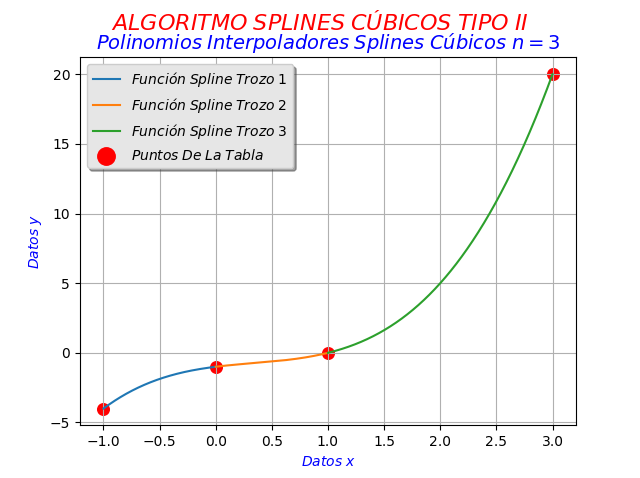
\includegraphics[width=8cm,height=5cm]{spline.png}
    \caption{Aproximación Spline Cúbica de Tipo II}
    \label{fig:spline}
\end{figure}\\
Te dejo como ejercicio que implementes con código Python el spline cúbico de tipo III, no es muy difícil realizarlo.
\section{Curvas Bézier}
Una de las mayores aplicaciones para dibujar de forma profesional en ordenador es el uso de las curvas de Bézier, pero para saber lo que son debes conocer antes el concepto de curva paramétrica.
\subsection*{Definición}
Una \textbf{Curva Paramétrica} en el plano euclídeo es una aplicación: $\alpha\,:\,[a,\;b]\subseteq\mathbb{R}\longrightarrow \mathbb{R}^2$ tal que $\alpha (t)=(x(t),\; y(t));\;\forall\; t\in\;[a,\; b]$. Una curva paramétrica no es mas que una forma alternativa de reescribir una curva. Tan sólo debes pensar en una recta, la puedes escribir en forma explícita $y=mx+n$, o en paramétricas, que es la curva paramétrica: $\alpha (t)=(x_0+v_1t,\;y_0+v_2t);\,\forall\,t\in\mathbb{R}$.\\ \\
Consideraremos una sucesión de puntos: $(x_0,\,y_0),\dots ,(x_n,\,y_n)$, un parámetro real $t\in [t_0,\,t_n]\;/\;t_0<\dots <t_n$. Construiremos funciones aproximación que cumplan: $x_i=x(t_i),\,y_i=y(t_i);\,i=0,\,1,\dots ,n$.\newpage
\subsection*{Curvas Bézier}
Podemos considerar una curva que viene definida por dos nodos: $(x_0,\,y_0),\,(x_1,\,y_1)$. A cada uno de estos nodos le consideramos sus respectivas rectas tangentes. A estas dos rectas tangentes las acotamos a sus respectivos segmentos de recta.\\
El segmento de recta asociado al primer nodo tendrá de extremos: $(x_0,\,y_0),\,(x_0+\alpha_0,\,y_0+\beta_0)$, y el otro segmento tendrá de nodos: $(x_1,\,y_1),\,(x_1+\alpha_1,\,y_1+\beta_1)$, con el parámetro $t\in [0,\,1]$. Los puntos $(x_0+\alpha_0,\,y_0+\beta_0),\,(x_1+\alpha_1,\,y_1+\beta_1)$ se denominan \textbf{Puntos Guía}. Al haber considerado rectas tangentes se cumple:
\[
\begin{Bmatrix}
x(0)=x_0 & x(1)=x_1\\
x^\prime (0)=\alpha_0 & x^\prime (1)=\alpha_1
\end{Bmatrix}\quad
\begin{Bmatrix}
y(0)=y_0 & y(1)=y_1\\
y^\prime (0)=\beta_0 & y^\prime (1)=\beta_1
\end{Bmatrix}
\]
Con todos estos datos podemos aplicar la interpolación de Hermite, obteniendo para cada componente de la curva paramétrica un polinomio aproximación de grado 3:
\[
x(t)=[2(x_0-x_1)+(\alpha_0 +\alpha_1)]t^3+[3(x_1-x_0)-(\alpha_1 +2\alpha_0)]t^2+\alpha_0 t+x_0
\]
\[
y(t)=[2(y_0-y_1)+(\beta_0 +\beta_1)]t^3+[3(y_1-y_0)-(\beta_1 +2\beta_0)]t^2+\beta_0 t+y_0
\]
Estos polinomios interpoladores cúbicos de Hermite si les incorporamos un factor 3 de escala reciben el nombre de \textbf{Polinomios Bézier} de nodos $(x_0,\,y_0),\,(x_1,\,y_1)$ con el parámetro real $t\in [0,\,1]$, aproximando una curva paramétrica $\alpha\,:\;[0,\,1]\longrightarrow \mathbb{R}^2$. Su expresión analítica es:
\[
x(t)=[2(x_0-x_1)+3(\alpha_0 +\alpha_1)]t^3+[3(x_1-x_0)-3(\alpha_1 +2\alpha_0)]t^2+3\alpha_0 t+x_0
\]
\[
y(t)=[2(y_0-y_1)+3(\beta_0 +\beta_1)]t^3+[3(y_1-y_0)-3(\beta_1 +2\beta_0)]t^2+3\beta_0 t+y_0
\]
Si consideramos $(x_0,\,y_0),\,(x_1,\,y_1),\dots ,(x_n,\,y_n)$, y cada dos nodos contiguos construimos sus respectivos polinomios Bézier, la unión de todos los polinomios Bézier forman una curva que recibe el nombre de \textbf{Curva Bézier}.\\
Hay que tener en cuenta que lo normal no es \textit{montar} a priori la curva Bézier. Lo corriente es que cuando hacemos un dibujo con software (como GIMP) se vayan calculando in situ las curvas de Bézier, ayudándonos con los puntos guía, como referencia, para ir cambiando la dirección de la curva. Al calcularse las curvas Bézier simultáneamente a lo que dibujamos necesitamos funciones con expresión analítica sencilla para los cálculos, así que un polinomio de grado pequeño es ideal, además para calcular las imágenes de los puntos de la curva se puede simplificar si lo hacemos con el algoritmo de Horner.
\subsection*{Ejemplo}
Los datos de la siguiente tabla aproximan la letra N, hacerlo mediante curvas de Bézier.
\begin{center}
    \begin{tabular}{|c||c|c|c|c|c|c|}
        \hline
        $i$ & $x_i$ & $y_i$ & $\alpha_i$ & $\beta_i$ & $\alpha^\prime _i$ & $\beta^\prime _i$ \\ \hline\hline
        0 & 3 & 6 & 3.3 & 6.5 & &  \\ \hline
        1 & 2 & 2 & 2.8 & 3 & 2.5 & 2.5 \\ \hline
        2 & 6 & 6 & 5.8 & 5 & 5 & 5.8\\ \hline
        3 & 5 & 2 & 5.5 & 2 & 4.5 & 2.5\\ \hline
        4 & 6.5 & 3 &  &  & 6.4 & 2.8\\ \hline
    \end{tabular}
\end{center}
\subsubsection*{Solución}
Lo haremos con un programa con un código Python utilizando curvas Bézier, para poder visualizarlo lo dibujaremos con ayuda de Matplotlib.
\begin{lstlisting}[frame=none]
import numpy as np
import matplotlib.pyplot as plt

def bezier(x, y, xx, yy, xxx, yyy):
    z = np.linspace(0, 1, 5000)
    plt.suptitle(r'$ALGORITMO\; DE\; BEZIER.$', fontsize=16, color='r')
    title = r'$Letra\; N\; Con\; Bezier$'
    plt.title(title, fontsize=14, color='b')
    plt.xlabel(r'$Datos\; x$', color='blue', fontsize=14)
    plt.ylabel(r'$Datos\; y$', color='blue', fontsize=14)
    for i in range(len(x) - 1):
        a_0 = x[i]
        b_0 = y[i]
        a_1 = 3 * (xx[i] - x[i])
        b_1 = 3 * (yy[i] - y[i])
        a_2 = 3 * (x[i] + xxx[i + 1] - 2 * xx[i])
        b_2 = 3 * (y[i] + yyy[i + 1] - 2 * yy[i])
        a_3 = x[i + 1] - x[i] + 3 * xx[i] - 3 * xxx[i + 1]
        b_3 = y[i + 1] - y[i] + 3 * yy[i] - 3 * yyy[i + 1]
        P = a_0  + a_1  * z + a_2  * z ** 2 + a_3  * z ** 3
        Q = b_0  + b_1  * z + b_2  * z ** 2 + b_3  * z ** 3
        plt.plot(P, Q, 'b-', lw=1.5)
    plt.show()

if __name__ == '__main__':
    x = np.array([3, 2, 6, 5, 6.5], dtype=float)
    y = np.array([6, 2, 6, 2, 3], dtype=float)
    xx = np.array([3.3, 2.8, 5.8, 5.5, np.nan], dtype=float)
    yy = np.array([6.5, 3, 5, 2, np.nan], dtype=float)
    xxx = np.array([np.nan, 2.5, 5, 4.5, 6.4], dtype=float)
    yyy = np.array([np.nan, 2.5, 5.8, 2.5, 2.8], dtype=float)
    bezier(x, y, xx, yy, xxx, yyy)
\end{lstlisting}
En la siguiente figura puedes ver la solución.
\begin{figure}[h!]
    \centering
    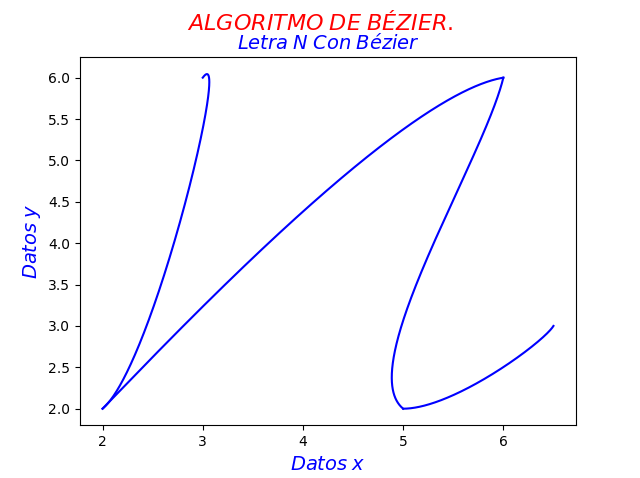
\includegraphics[width=8cm,height=5cm]{BezierN.png}
    \caption{Curva Bézier Letra N}
    \label{fig:spline}
\end{figure}\\
En el código si borramos las pocas líneas dedicadas para dibujar obtenemos el algoritmo para curvas Bézier cúbicas.
\section{Bibliografía}
MÉTODOS NUMÉRICOS, Teoría, problemas y prácticas con MATLAB --- Juan Antonio Infante Del Río, José María Rey Cabezas. EDITORIAL: Pirámide. 3ª Edición.\\
NUMERICAL ANALYSIS --- Richard L. Burden, J. Douglas Faires. 9th edition.
\end{document}